Two equal masses are connected by a string that hangs over two pulleys (of negligible size), as shown in Fig. 1.6. The left mass moves in a vertical line, but the right mass is free to swing back and forth in the plane of the masses and pulleys. It can be shown (see Problem 6.4) that the equations of motion for $r$ and $\theta$ (labeled in the figure) are
\begin{equation*}
2\ddot{r} = r\dot{\theta}^{2} - g(1 - \cos\theta),
\end{equation*}
\begin{equation*}
\ddot{\theta} = -\frac{2\dot{r}\dot{\theta}}{r} - \frac{g\sin\theta}{r}. \tag{1.16}
\end{equation*}

Assume that both masses start out at rest, with the right mass making an initial angle of $10^{\circ} = \pi/18$ with the vertical. If the initial value of $r$ is 1 m, how much time does it take for it to reach a length of 2 m? Write a program to solve this numerically. Use $g = 9.8 \,\text{m/s}^{2}$.

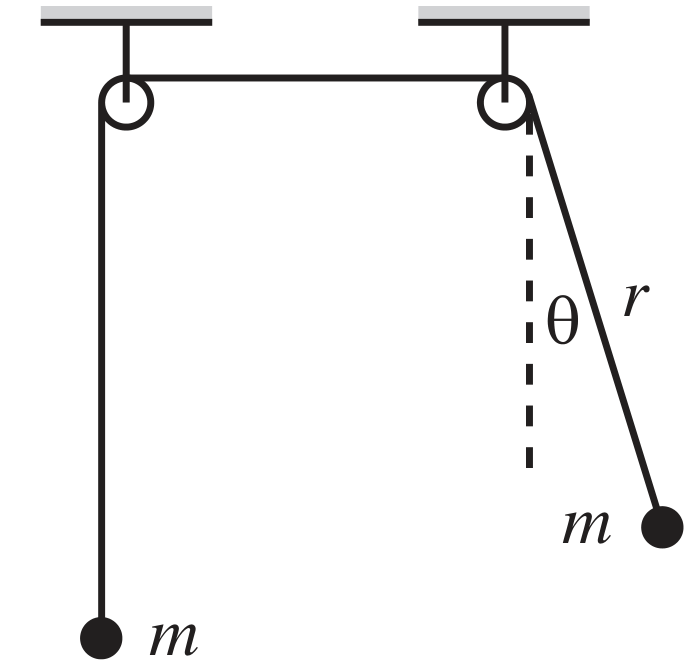
\includegraphics[width=\linewidth]{figures/qfig1.png}